
% \begin{figure}[t]
% % \label{fix:exp-results}
%   \centering

%   \begin{subfigure}[b]{0.6\columnwidth}
%     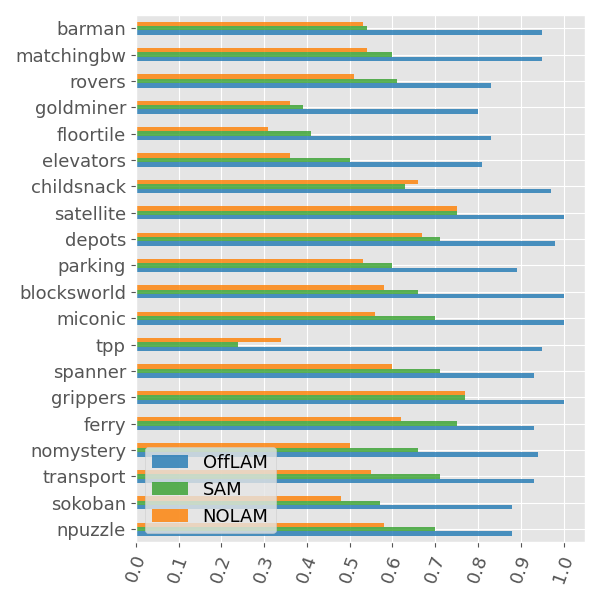
\includegraphics[width=\textwidth]{figures/10_traces_mini/syn_precision.png}
%     \caption{Syntactic precision}
%   \end{subfigure}
%   \\
%   % \begin{subfigure}[b]{0.24\textwidth}
%   %   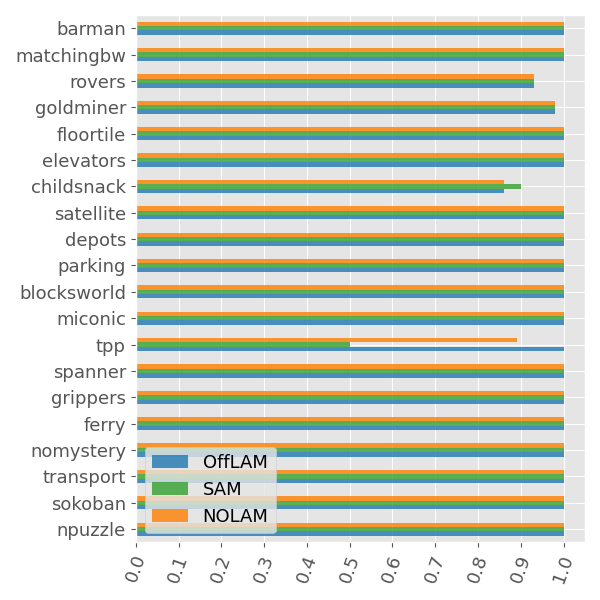
\includegraphics[width=\textwidth]{figures/10_traces_mini/syn_recall.png}
%   %   \caption{Syntactic recall}
%   % \end{subfigure}
%   \begin{subfigure}[b]{0.6\columnwidth}
%     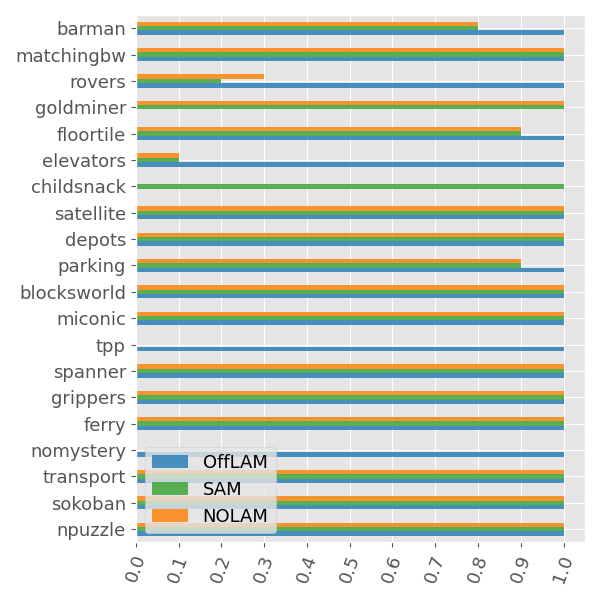
\includegraphics[width=\textwidth]{figures/10_traces_mini/solving.png}
%     \caption{Problem solving ratio}
%   \end{subfigure}
%   \\
%   \begin{subfigure}[b]{0.6\columnwidth}
%     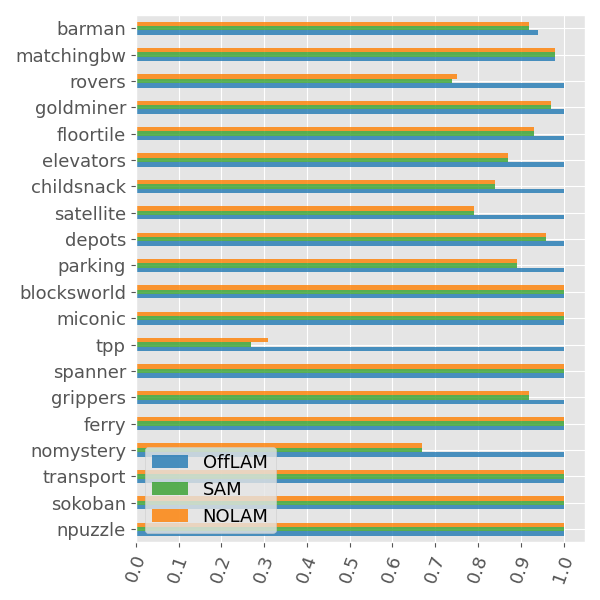
\includegraphics[width=\textwidth]{figures/10_traces_mini/app_recall.png}
%     \caption{Applicability recall}
%   \end{subfigure}




%   \caption{Evaluation metrics when learning from a training set $\Ttrain$ with $10$ traces for every domain.}
%   \label{fig:exp-mini}
% \end{figure} 


% OPTION B

\begin{figure}[ht]
% \label{fix:exp-results}
  \centering

  \begin{subfigure}[b]{\columnwidth}
    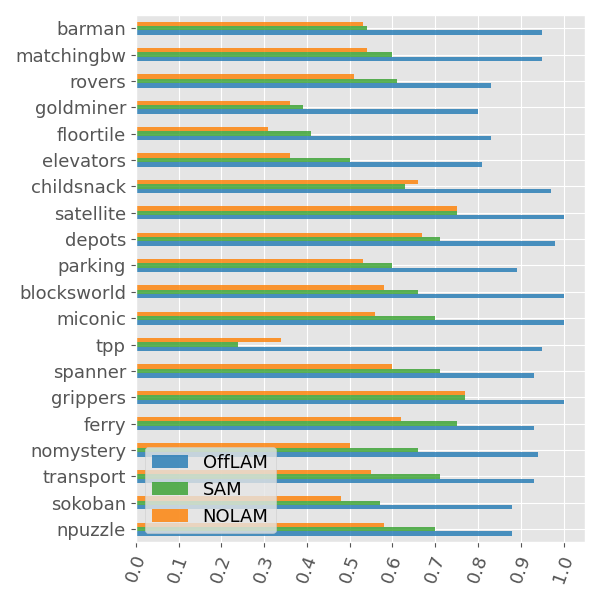
\includegraphics[width=\textwidth]{figures/10_traces_mini/syn_precision.png}
    \caption{Preconditions syntactic precision}
    \label{fig:syn-precision}
  \end{subfigure}
  \hfill
  % \begin{subfigure}[b]{0.24\textwidth}
  %   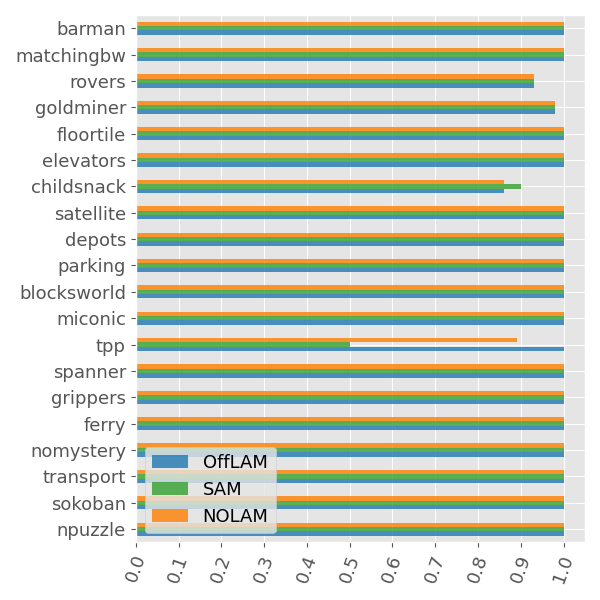
\includegraphics[width=\textwidth]{figures/10_traces_mini/syn_recall.png}
  %   \caption{Syntactic recall}
  % \end{subfigure}
  \begin{subfigure}[b]{\columnwidth}
    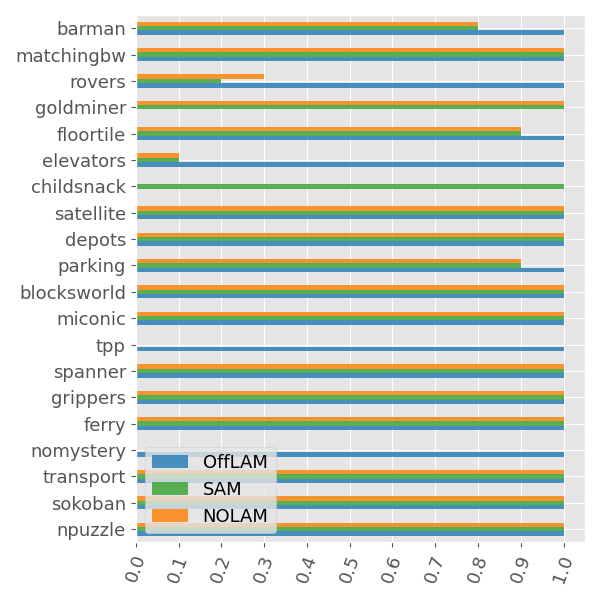
\includegraphics[width=\textwidth]{figures/10_traces_mini/solving.png}
    \caption{Problem solving ratio}
    \label{fig:solving-ratio}
  \end{subfigure}
  \hfill
  \begin{subfigure}[b]{\columnwidth}
    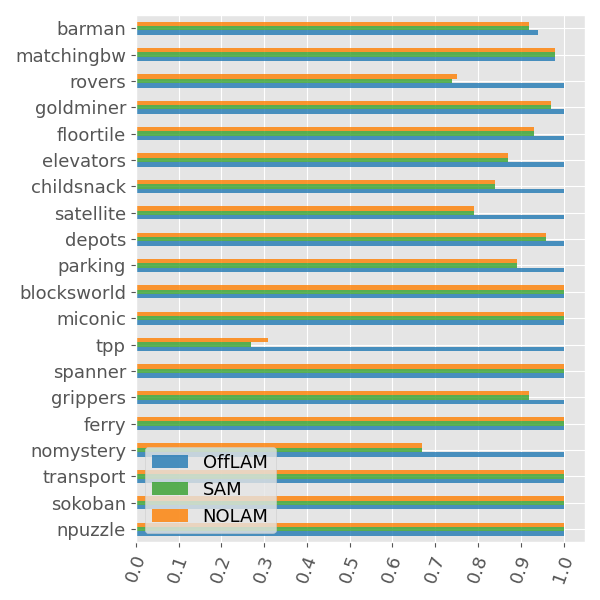
\includegraphics[width=\textwidth]{figures/10_traces_mini/app_recall.png}
    \caption{Applicability recall}
  \end{subfigure}




  \caption{Evaluation metrics for the models learned by \samshort{}, \offlam{} and \nolam{} from a training set $\Ttrain$ of $10$ traces for every domain.}
  \label{fig:exp-mini}
\end{figure} 